\newpage
\section{Kierownik projektu}
Jako rozwinięcie części teoretycznej zarządzania projektami kluczowym jest zrozumienie roli oraz zadań kierownika projektu. Dodatkowo w literaturze przedmiotu jest dostępnych wiele badań oraz prac omawiających cechy oraz kompetencje kierownika projektu. Warto przytoczyć te teksty w celu udzielenia trafniejszej odpowiedzi na postawione w pracy pytanie.

\subsection{Kierownik projektu}
Najprostsza definicja za pomocą, której można wyjaśnić kim jest kierownik projektu to: osoba, która wyznacza proces dostarczenia zmiany i jest odpowiedzialna za zarządzanie tym procesem \autocite{Turner2016}.
Bardziej powszechne wydaje się jednak rozumienie kierownika jako podmiotu odpowiedzialnego za realizację projektu w sposób bezpieczny, zgodny z harmonogramem i budżetem oraz osiągający wymagane standardy wydajności lub jakości określone przez klienta \autocite{Sommerville}.
Nicholas i Steyn podają w swojej książce jednak bardziej metaforyczne rozumienie kierownika projektu jako swoistego spoiwa scalającego wszystkie elementy projektu oraz napędzającego jego rozwój. W ramach tej funkcji pełnione są liczne zadania, między innymi integracja, komunikacja, podejmowanie decyzji, motywowanie, propagowanie idei, działalność przedsiębiorcza oraz inicjowanie zmian. \autocite{NicholasSteyn}
Z taką definicją kierownika projektu zgadza się również Blackburn i Sarah. W swoim artykule określili kierownika projektu jako byt łączący sieć aktorów w celu realizacji wspólnego celu \autocite{BlackburnSarah}

\subsection{Role i zadania kierownika projektu}
Zgodnie z przytoczonymi definicjami kierownika projektu, jego głównym zadaniem jest zapewnienie dostarczenia końcowego produktu w ramach przyjętego budżetu i ustalonych terminów, zgodnie z określonymi wymaganiami technicznymi. Pozostałe obowiązki ulegają modyfikacji w zależności od umiejętności kierownika, etapu realizacji przedsięwzięcia, rozmiaru i charakteru projektu oraz zakresu odpowiedzialności przekazanej przez wyższe kierownictwo.
Mimo zróżnicowania kompetencji, zakres obowiązków zazwyczaj obejmuje:
\begin{itemize}
    \item Opracowanie planu działań projektowych, zadań oraz końcowych rezultatów, co obejmuje sporządzenie struktury podziału pracy, ustalenie harmonogramu i budżetu, a także koordynację zadań oraz dystrybucję zasobów. Polega to na łączeniu różnorodnych działań i rozproszonych elementów w sposób umożliwiający osiągnięcie wyznaczonych celów czasowych, budżetowych i jakościowych. Centralną funkcją kierownika projektu jest zapewnienie spójności wszystkich składników przedsięwzięcia, co umożliwia ich harmonijną współpracę zgodnie z ustalonym planem.
    \item Dobór oraz organizacja zespołu odpowiedzialnego za realizację przedsięwzięcia. Nawet przy ograniczonych formalnych uprawnieniach do podejmowania decyzji kadrowych, rola ta umożliwia wywieranie znaczącego wpływu na dokonywane wybory osób dysponujących odpowiednimi kompetencjami.
    \item Nawiązywanie kontaktów z interesariuszami oraz oddziaływanie na ich postawy. Na styku licznych kanałów informacyjnych znajduje się rola kierownika, odpowiedzialnego za zbieranie oraz dystrybucję danych – obejmujących raporty, zgłoszenia, notatki służbowe czy skargi. Przekazywane informacje są starannie opracowywane i poddawane analizie, aby wszyscy interesariusze byli rzetelnie poinformowani o założeniach dotyczących polityki, celów, budżetów, harmonogramów, wymagań, postępów prac oraz zmian w projekcie.
    \item Prowadzenie negocjacji oraz scalanie działań kierowników działów, wykonawców, użytkowników i kadry zarządzającej. Istotnym aspektem działalności kierownika jest również propagowanie idei projektu, co wiąże się z kreowaniem przekonania o jego wartości i wykonalności. W początkowej fazie koncepcyjnej to właśnie kierownik często dysponuje pełnym obrazem przedsięwzięcia, a jego zdolność do zdobycia poparcia kluczowych interesariuszy może przesądzić o uzyskaniu niezbędnego finansowania
    \item Zapewnienie kanału komunikacji z klientem. Znaczenie tej komunikacji podkreślają w swojej pracy Turner i MUller \autocite{turnermuller}. Przypominają oni, że kierownik projektu działa tak naprawdę w imieniu i na rzecz klienta, a więc projekt powinien być zgodny z jego potrzebami.
    \item Nadzór nad postępem realizacji projektu. Ocena rzeczywistych osiągnięć technicznych w porównaniu z planowanymi, przegląd i weryfikacja zasadności celów technicznych, potwierdzenie ciągłej potrzeby realizacji projektu, nadzorowanie wydatków na zasoby oraz porównanie przewidywanej wartości z poniesionymi kosztami. \autocite{Roman}\autocite{vaupel}
    \item Identyfikacja problemów o podłożu technicznym i funkcjonalnym a następnie bezpośrednie ich rozwiązywanie lub poszukiwanie adekwatnego wsparcia. Zarządzanie ryzykiem jest integralną częścią zarządzania projektem, obejmującą identyfikację, ocenę i planowanie reakcji na ryzyka w celu minimalizacji ich wpływu. W większych projektach, gdzie ryzyko i konsekwencje są znaczące, skuteczne zarządzanie ryzykiem może decydować o sukcesie lub porażce przedsięwzięcia.
    \item Radzenie sobie z sytuacjami kryzysowymi oraz rozwiązywanie pojawiających się konfliktów. Determinacja i skupienie zespołu na wspólnym celu stanowią jeden z kluczowych czynników mobilizujących do działania. W strukturze organizacyjnej projektu to właśnie kierownik odpowiada za kreowanie poczucia wspólnego kierunku i zaangażowania. Pomimo występowania licznych czynników sprzyjających motywacji, takich jak spontaniczność, osiągnięcia czy entuzjazm, utrzymanie wysokiego poziomu zaangażowania bywa trudne w długotrwałych i wymagających przedsięwzięciach. Czynniki takie jak brak wcześniejszych wzorców, praca na niepełny etat, różnorodność specjalizacji, sporadyczność kontaktów oraz dystans przestrzenny mogą znacząco wpływać na spadek motywacji. Skuteczne zarządzanie projektem wymaga jednak zdolności do budowania entuzjazmu, ducha zespołu, pewności siebie oraz dążenia do doskonałości.
    \item Sugerowanie zakończenia projektu lub zmiany kierunku działań, gdy założone cele okazują się nieosiągalne. Centralne położenie kierownika umożliwia podejmowanie decyzji związanych z alokacją zasobów, definiowaniem zakresu działań oraz równoważeniem kryteriów harmonogramu, kosztów i jakości. \autocite{NicholasSteyn}
\end{itemize}

Ciekawa interpretacja roli oraz zadań kierownika projektu została również przedstawiona na rysunku 3.1. Autorzy zwracają większą uwagę na rolę interpersonalną kierownika projektu i określają go w tym kontekście jako mentora, mediatora, psychologa i lidera.
\begin{figure}
\caption{Role kierownika projektu}
\centering
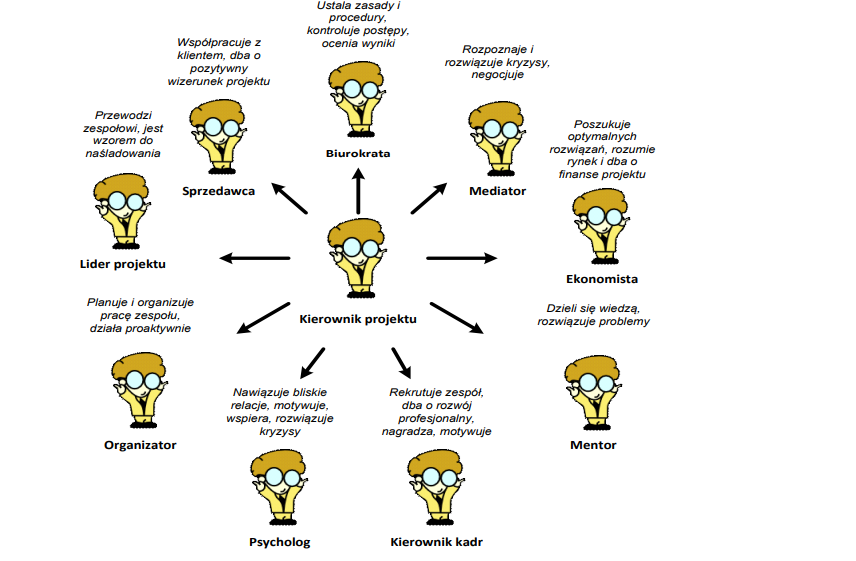
\includegraphics[width=14cm]{img/rola.png}
\caption*{Źródło: Wykład \textit{Podstawy Zarządzania Projektami}, M. Juchniewicz}
\end{figure}

\subsection{Kompetencje kierownika projektu}
Dywagacje na temat kompetencji, jakie powinien posiadać kierownik projektu, stały się zagadnieniem często poruszanym w literaturze przedmiotu. Jednak nie tylko wiedza i umiejętności techniczne mają znaczenie. Menedżerowie są bardziej skłonni do osiągania lepszych wyników lub pozostawania dłużej na swoim stanowisku, jeśli ich cechy osobiste odpowiadają wymaganiom stanowiska.\autocite{MUMFORD200011}
Na rysunkach 3.2. oraz 3.3. zostały przedstawione wyniki dostępnych badań.
Na podstawie analizy dostępnej literatury i badań w dalszych sekcjach według ważności zostały wymienione kluczowe kompetencje: \autocite{analizaMulti} \autocite{Alvarenga} \autocite{arras2010} \autocite{ziek} \autocite{brill} \autocite{arras2015}

\begin{table}
    \caption{Kompetencje kierowników według raportu Arras}
    \centering
    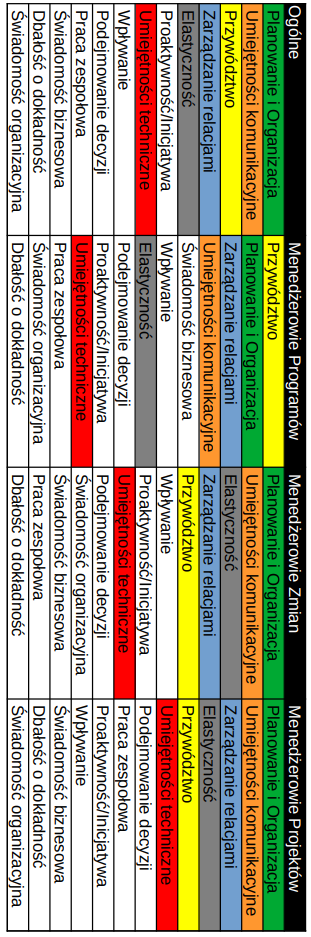
\includegraphics[width=0.45\linewidth]{arras.png}
    \caption*{Źródło: Arras People Project Management Benchmark Report 2010 }
  \end{table}


    \begin{table}[ht!]
        \centering
        \caption{Analiza częstotliwości występowania kompetencji kierowników projektów}
        \begin{tabular}{>{\raggedright\arraybackslash}p{0.5cm} >{\raggedright\arraybackslash}p{4.5cm} >{\centering\arraybackslash}p{1.2cm} >{\centering\arraybackslash}p{1.2cm} >{\raggedright\arraybackslash}p{6cm}}
        \toprule
        \textbf{Poz.} & \textbf{Kompetencja} & \textbf{Liczba} & \textbf{\% wystąpień} & \textbf{Opis/Przykład} \\
        \midrule
        1 & Wiedza specjalistyczna branżowa & 1288 & 56\% & Wymaga umiejętności technicznych właściwych dla danej branży (np. programowanie, znajomość języka, kwalifikacje inżynierskie, wiedza księgowa, itp.) \\
        \rowcolor[gray]{0.95}
        2 & Umiejętności komunikacyjne & 1078 & 47\% & Niezbędne umiejętności komunikacyjne \\
        3 & Umiejętności zarządzania zespołem & 907 & 39\% & Zarządzanie zespołem \\
        \rowcolor[gray]{0.95}
        4 & Zdolności przywódcze & 694 & 30\% & Potrafi prowadzić zespół \\
        5 & Wykształcenie wyższe & 682 & 30\% & Wykształcenie wyższe \\
        \rowcolor[gray]{0.95}
        6 & Zarządzanie interesariuszami & 656 & 28\% & Zarządzanie oczekiwaniami interesariuszy \\
        7 & Zarządzanie budżetem & 654 & 28\% & Zarządzanie budżetem projektu zgodnie z celami \\
        \rowcolor[gray]{0.95}
        8 & Zarządzanie harmonogramem & 653 & 28\% & Zapewnienie realizacji projektu zgodnie z harmonogramem \\
        9 & Świadomość biznesowa & 488 & 21\% & Zorientowanie na biznes/przedsiębiorczość \\
        \rowcolor[gray]{0.95}
        10 & Praca zespołowa & 458 & 20\% & Praca w zespole w strukturze macierzowej \\
        \bottomrule
        \end{tabular}
        \caption*{Zródło: A Multidimensional Analysis of ProjectManager Competences Maxwell Chipulu, Jun Guan Neoh, Udechukwu (Udi) Ojiako, and Terry Williams 2013}
        \end{table}


\subsubsection{Komunikacja}
W najnowszych badaniach oraz pracach kluczowe okazują się umiejętności interpersonalne.\autocite{brill}. Umiejętności komunikacyjne są kluczowe w różnych kontekstach: negocjacje, komunikacja, relacje z klientami i zarządzanie konfliktem. Literatura opisuje komunikację jako podstawowe narzędzie dla kierownika projektu w jego kluczowej funkcji łączenia i pośredniczenia między wieloma podmiotami zaangażowanymi w projekt: zespołem, sponsorami, sprzedawcami, kierownikami funkcjonalnymi, użytkownikami i klientami oraz innymi interesariuszami. Wyraźnie wynika z tego, że to właśnie kompetencje komunikacyjne pozwalają kierownikom projektów być skutecznymi i mieć wpływ na sukces projektu. \autocite{Alvarenga}

Ziek oraz Anderson w swojej pracy podkreślają, że rola komunikacji w projekcie to nie jest jedynie czynnik wpływający na sukces bądź porażkę projektu. Uważają oni, że jest to fundament zarządzania projektami. Zrozumienie roli komunikacji zapewnia kierownikom projektów dodatkowe środki kontroli nad projektem, wykraczające poza budżety i harmonogramy.\autocite{ziek}

\subsubsection{Przywództwo}
Podążając za Burnsem, przywództwo jest „jednym z najczęściej obserwowanych i najmniej rozumianych zjawisk na ziemi”\autocite{burns}. W związku ze skomplikowaną naturą tej cechy nie jest ona łatwa w wyjaśnieniu. Tabassi i Bakar zidentyfikowali kluczowe komponenty związane ze zjawiskiem przywództwa i zdefiniowali je jako proces, w którym lider ze swoją inteligencją i siłą woli ma wpływ na grupę podwładnych, aby móc rozwijać ich potencjały w celu osiągnięcia celów organizacyjnych w wyznaczonym czasie, finansowaniu i jakości.\autocite{Tabassi} 

Kierownik projektu nie może ograniczać się jedynie do zarządzania harmonogramem i zadaniami – kluczowe stają się rozwinięte kompetencje przywódcze, które są fundamentem sukcesu całego przedsięwzięcia. W projektach, w których nieuniknione są kryzysy i konflikty, zdolność szybkiego podejmowania decyzji oraz umiejętność skutecznego komunikowania się z zespołem nabierają szczególnego znaczenia. Nicholas podkreśla, że to właśnie przywództwo jest jedną z czterech funkcji kierownika, który ukierunkowuje pracę swoich pracowników oraz motywuje ich do realizacji wspólnego celu. \autocite{NicholasSteyn} 
W badaniu Alvarenga cechy przywódcze zostały uznane za najważniejszą kompetencję u kierownika projektu.\autocite{Alvarenga}

\subsubsection{Zarządzanie sobą (ang. Self-management)}
Kompetencje zarządzania sobą obejmują wizję, poznanie, odporność emocjonalną, samoświadomość. Odzwierciedlają one potrzebę kierowników projektów, którzy są oddani samorozwojowi i ciągłemu uczeniu się. Odporność emocjonalna jest również bardzo istotna dla kierowników projektów: ciągła presja, niepewność, ryzyko, konflikty zespołowe i inne codzienne wyzwania mogą prowadzić do stresu, a w skrajnych sytuacjach do wypalenia zawodowego.\autocite{Alvarenga} Samoświadomość oraz odporność emocjonalna są również podkreślane jako kluczowe cechy kierownika projektu w pracy Turnera i Mullera. Według ich badań samoświadomość jest zwłaszcza szczególnie ważna w projektach o średniej złożoności.\autocite{turnermuller2010}

\subsubsection{Umiejętności zarządcze}
Kierownik projektu musi zdecydować, jak przydzielić zasoby ludzkie, finansowe i informacyjne do różnych zadań projektu. Kompetencja ta opiera się na planowaniu, organizowaniu, koordynowaniu i kontrolowaniu zadań.\autocite{Gottschalk} Znaczenie tych umiejętności podkreślają również w swojej pracy Udo i Koppensteiner. Według nich kierownik projektu musi znać podstawy procesów zarządzania projektami, metodologie, narzędzia i techniki oraz potrafić dostosować je do organizacji.
Jednym ze sposobów na sprawdzenie tych kompetencji jest certyfikacja bądź odpowiednie studia.\autocite{Koppensteiner} Odpowiednie wykształcenie pojawiło się również w wynikach badań IEEE, aż 30\% respondentów uznało stopień naukowy z dziedziny zarządzania za istotną cechę kierownika projektu.\autocite{analizaMulti}

\subsubsection{Umiejętności techniczne}
Kolejną kompetencją kierownika projektu, która często pojawia się w literaturze, są umiejętności techniczne rozumiane jako wiedza domenowa oraz znajomość narzędzi potrzebnych w zarządzaniu projektami. \autocite{arras2010} \autocite{brill}
Znajomość domeny i wiedzy specyficznej dla branży jest cenna, gdyż to kierownik projektu identyfikuje potrzeby użytkowników i opracowuje rozwiązania, które zmieniają sytuacje biznesowe. Główną odpowiedzialnością kierownika projektu jest zapewnienie, że szybko planowane zmiany są zrozumiane, zaplanowane, wdrożone i strategicznie wykorzystane w organizacji.\autocite{Gottschalk} Nie byłby on w stanie tego osiągnąć bez dobrego zrozumienia projektu oraz działań wykonywanych w ramach projektu.
Ciekawym opisem poziomu kompetencji technicznych kierownika projektu jest podejście zaproponowane przez Nicholasa. Tłumaczy on, że kompetencje kierownika powinny pokrywać cały zakres projektu, ale ograniczając go jedynie do pierwszego poziomu struktury podziału pracy (ang. Work breakdown structure, WBS).\autocite{NicholasSteyn}

\subsection{Znaczenie wiedzy z zakresu inżynierii oprogramowania dla kierownika projektu}
Aby podejmować świadome decyzje, kierownicy projektów muszą rozumieć aspekty techniczne projektu. Ich kompetencje powinny obejmować pełny zakres projektu. W środowiskach nisko- lub nietechnologicznych tę znajomość można rozwijać poprzez doświadczenie i szkolenia nieformalne. W projektach o wysokim zaawansowaniu technologicznym wymagania są surowsze i zwykle obejmują karierę ukształtowaną w środowisku technologicznym oraz wiedzę z zakresu nauki lub inżynierii.

Choć kierownicy projektów rzadko przeprowadzają analizy techniczne, muszą być wykwalifikowani do podejmowania ocen technicznych oraz zdolni do analizy i integracji pracy oraz wiedzy. Wielu specjalistów technicznych nie radzi sobie dobrze ze współpracą z innymi, ponieważ większość kształcenia w dziedzinie inżynierii i technologii kładzie nacisk na analizę, pomijając umiejętności pracy zespołowej. Aby skutecznie komunikować się ze wszystkimi uczestnikami projektu i integrować ich pracę, kierownik projektu musi rozumieć i posługiwać się językiem specjalistów technicznych.\autocite{NicholasSteyn}

Z takim postrzeganiem polemizuje jednak badanie przeprowadzone wśród brazylijskich kierowników projektów informatycznych.\autocite{silva2015project} Było to jakościowe badanie eksploracyjne z udziałem 16 brazylijskich profesjonalistów IT z różnych sektorów.
Wbrew tradycyjnemu postrzeganiu w środowisku projektów informatycznych, umiejętności z zakresu inżynierii oprogramowania uznano za mniej istotne niż kompetencje behawioralne, biznesowe i menedżerskie. Analiza wykazała, że najważniejsze kompetencje to:
\begin{itemize}
    \item zarządzanie zespołem,
    \item wiedza domenowa,
    \item komunikacja,
    \item zarządzanie projektami,
    \item umiejętności interpersonalne.
\end{itemize}
\autocite{silva2015project}

Kategorie takie jak zarządzanie zespołem, wiedza domenowa, umiejętności interpersonalne i komunikacja zebrały łącznie 349 wzmianek, podczas gdy umiejętności z zakresu inżynierii oprogramowania – jedynie 5. Dla respondentów kompetencje związane z relacjami i biznesem są więc kluczowe dla sukcesu projektu informatycznego. Niektórzy zauważyli nawet, że kierownicy z silnym profilem technicznym mogą bagatelizować inne aspekty zarządzania, takie jak strategia organizacyjna, umiejętności polityczne czy zarządzanie ludźmi. W badaniu została przytoczona w tym kontekście wypowiedź respondentów:
\begin{itemize}
    \item"Był bardziej techniczny, brakowało mu wiedzy politycznej. Brakowało mu politycznej siły, by projekt działał."
    \item"Czasami kierownik z dobrymi umiejętnościami technicznymi nie skupia się na ludziach." 
\end{itemize}

Badanie jednak nie bagatelizuje całkowicie roli umiejętności z zakresu inżynierii oprogramowania, uznaje je za "niezbędne, ale niewystarczające". Niektórzy z respondentów badania podkreślali, że wiedza techniczna ułatwia komunikację z programistami oraz usprawnia zarządzanie projektem. Przytoczono w tym kontekście następujące wypowiedzi.
\begin{itemize}
    \item"Gdy masz umiejętności techniczne, możesz porozumieć się z osobą rozwijającą system i przekazać programiście oczekiwania klienta."
    \item"Jeśli kierownik nie ma wiedzy technicznej, musi stale polegać na kimś, kto ją posiada."    
\end{itemize}

Zgromadzone dane wskazują, że umiejętności z zakresu inżynierii oprogramowania nie wystarczą, aby zapewnić pozytywne rezultaty w zarządzaniu projektami. Nie oznacza to, że kierownicy projektów IT powinni porzucić kompetencje techniczne wypracowane w trakcie kariery. Sugeruje to jednak, że powinni łączyć umiejętności techniczne z kompetencjami interpersonalnymi i menedżerskimi, aby skuteczniej osiągać sukces projektu.\autocite{silva2015project}


Podobne badania przeprowadził Stevenson wśród osób odpowiedzialnych za rekrutację kierowników projektów informatycznych.\autocite{stevenson2010pm} Badanie to wykazało niską ocenę ekspertyzy technicznej jako kompetencji kierowników projektów. Biorąc pod uwagę zmiany i konsolidację ról w zespołach projektowych oraz trend wzrostowy zatrudniania kierowników o profilu technicznym w ciągu ostatniej dekady, oczekiwano, że umiejętności techniczne zostaną uznane za istotne kryterium. Jedną z interpretacji tych wyników jest to, że firmy mniej cenią kompetencje techniczne kierowników projektów zdobyte w innych firmach, a bardziej skupiają się na szkoleniu swoich pracowników wewnętrznie, w oparciu o własną technologię. Inna interpretacja zakłada, że respondenci uważali, iż podstawowy poziom wiedzy technicznej jest inherentny u wszystkich kandydatów, więc nie traktowali go jako kryterium różnicującego talenty.

Wyniki badania jednoznacznie wskazują, że kompetencje „miękkie” takie jak przywództwo, umiejętność komunikacji na wielu poziomach, zdolności werbalne i pisemne, postawa oraz zdolność radzenia sobie z niejednoznacznością i zmianami – są kluczowymi cechami, które są poszukiwane wśród kierowników projektów informatycznych i które decydują o skutecznym zarządzaniu projektami.\autocite{stevenson2010pm}

Ważność umiejętności technicznych a menedżerskich zależy od typu projektu. W projektach innowacyjnych kierownik musi mieć wyższe kompetencje techniczne ze względu na złożoność problemów i techniczne nastawienie zespołu. W projektach rozwojowych lub nietechnicznych kluczowe są zdolności menedżerskie ze względu na współpracę z wieloma obszarami funkcjonalnymi. Ogólnie rzecz biorąc, kierownicy muszą mieć wystarczające umiejętności techniczne, by rozumieć problem, choć nadmierne skupienie na umiejętnościach technicznych może prowadzić do zaniedbywania roli menedżerskiej. Nie ma jednak substytutu dla silnych kompetencji zarządczych w tej roli.

Aby sprostać wymaganiom zarówno technicznym, jak i administracyjnym, w projektach czasem zatrudnia się dwóch menedżerów: technicznego i administracyjnego. Często występuje to w projektach budowlanych, gdzie architekt odpowiada za kwestie techniczne, a tzw. kierownik projektu zajmuje się „dokumentacją administracyjną”. Obecność dwóch menedżerów komplikuje koordynację, komunikację i kwestie władzy, ponieważ obaj dzielą odpowiedzialność. Co więcej, gdy kierownik projektu jest podporządkowany architektowi, jego zdolność do zarządzania projektem jest ograniczona. Podobny podział występuje w branży filmowej: producent zarządza zasobami, harmonogramami i budżetami (pełniąc rolę kierownika projektu), podczas gdy reżyser nadzoruje kwestie techniczno-artystyczne. Ponieważ tworzenie filmu to przedsięwzięcie artystyczne, reżyserzy potrzebują elastyczności w budżetach i harmonogramach zdjęć, ale koszty również mają znaczenie – producent staje przed dylematem: „jaką cenę zapłacić za kreatywność?”.

Idealnie, projekt powinien mieć jednego kierownika, a wszyscy inni pełniący role menedżerskie lub administracyjne podlegają jemu.\autocite{NicholasSteyn}